\documentclass[11pt]{article}
\usepackage[margin=1in]{geometry}
\usepackage{amsmath,amssymb,amsthm,booktabs,graphicx}
\usepackage[hidelinks]{hyperref}
\usepackage{url}
\numberwithin{equation}{section}
\newtheorem{theorem}{Theorem}[section]
\newtheorem{lemma}[theorem]{Lemma}
\newtheorem{proposition}[theorem]{Proposition}
\newtheorem{corollary}[theorem]{Corollary}
\theoremstyle{definition}
\newtheorem{definition}[theorem]{Definition}
\theoremstyle{remark}
\newtheorem{remark}[theorem]{Remark}
\newcommand{\R}{\mathbb{R}}
\newcommand{\C}{\mathbb{C}}
\newcommand{\Z}{\mathbb{Z}}
\newcommand{\floor}[1]{\lfloor #1\rfloor}
\DeclareRobustCommand{\code}[1]{\path{#1}}
\DeclareRobustCommand{\lean}[1]{\path{#1}}
\makeatletter\g@addto@macro{\UrlBreaks}{\do\_}\makeatother
\newcommand{\status}[1]{\textsf{[#1]}}

\title{The regular $n$-gon of point vortices is stable at its bifurcation point:\\
Montaldi--Tokieda's Conjecture~13 for every $n\ge4$}
\author{Gordon Speagle\\
Independent Researcher, Boise, ID, USA\\
\texttt{gspeagle@gmail.com}}
\date{Draft, 23 October 2026}

\begin{document}
\emergencystretch=1em
\maketitle

\begin{abstract}
Montaldi and Tokieda put point vortices on the sphere, the plane and the hyperbolic plane into one
family of geometries and showed that a regular ring of $n\ge4$ identical vortices loses stability at an
explicit value $b_n$ of the curvature parameter. They conjectured that the ring is still stable \emph{at}
$b_n$ (their Conjecture~13). We prove this for every $n\ge4$. At $b_n$ the reduced Hamiltonian has a
degenerate critical point whose Hessian is positive semidefinite with a one- or two-dimensional kernel,
so stability is decided by a quartic coefficient $c_4$. We compute $c_4$ on the momentum level set, in
closed form for all $n$:
\begin{gather*}
c_4=\frac{(n-2)\,(m^4+40m^2+48m+16)}{192\,n(n-1)}\quad(n\text{ even},\ m=n-2),\\
c_4=\frac{(n-1)(n-3)(n^2-9n+38)}{128\,n}\quad(n\text{ odd}),
\end{gather*}
both positive. A standard energy--momentum argument for degenerate minima then gives Lyapunov stability
modulo rotations. Working on the level set matters: the level set bends at second order into a direction
where the Hessian is not zero, and this bending contributes at fourth order. For even $n$, Montaldi and
Tokieda expand along a straight line that leaves the level set. Their quartic has the right sign but not
the right value: at $n=4$ the $t^4$ coefficient along their line is $6-4\sqrt3/3\approx3.69$, while the
level set gives $4$. The
algebra and the series coefficients (the closed forms, positivity, the Taylor coefficients derived
from the Hamiltonian, the root-of-unity sums, the Fourier blocks of the Hessian, the comparison with the
straight line), and the abstract Lyapunov lemmas, are checked in Lean~4. Reducing the problem to these statements, and instantiating the
abstract argument for the vortex flow, are done by hand. No human specialist has refereed the proof.
\end{abstract}

\tableofcontents

%======================================================================
\section{Introduction}\label{sec:intro}
%======================================================================

\paragraph{The question.} A ring of $n$ identical point vortices placed at the vertices of a regular
polygon rotates rigidly. Whether this rotating ring is stable is one of the oldest questions in vortex
dynamics: Thomson~\cite{Thomson} found that in the plane the ring is linearly stable for $n\le6$, unstable
for $n\ge8$, and degenerate for $n=7$. The heptagon was shown to be nonlinearly stable much
later~\cite{KY,Schmidt}. On a sphere the answer depends on latitude, and on the hyperbolic plane on the
radius.

Montaldi and Tokieda~\cite{MT} (``MT'') put the sphere, the plane and the hyperbolic plane into a single
one-parameter family of geometries. In it the ring's stability is governed by one number,
$b=\lambda r_0^2$ (curvature times squared radius, in their normalisation). They prove that for $n\ge4$
the ring is stable for $b<b_n$ and unstable for $b>b_n$, where $b_n$ is explicit (equation~\eqref{eq:bn}
below), and that a pitchfork bifurcation occurs at $b_n$. The threshold $b_n$ lies on the sphere for
$n=4,5,6$, is the plane ($b_7=0$, Thomson's heptagon) for $n=7$, and lies on the hyperbolic plane for
$n\ge8$. At the bifurcation point itself the linearisation is degenerate, so stability is a nonlinear
question. MT state (\cite[p.~23]{MT}, arXiv:1210.5662v1):

\begin{quote}
\textbf{Conjecture 13.} \emph{For all values of $n$, the $n$-gon is stable at the bifurcation point.}
Above, we have proved this for all even $n$ and for $n=3,5,7,9,11$.
\end{quote}

Here ``stable'' means Lyapunov stability modulo the rotations about the ring's centre~\cite[pp.~10,
15]{MT}. MT treat odd $n=5,9,11$ by floating-point evaluation of three coefficients, $n=7$ by computer
algebra, and even $n$ by a closed-form computation of a quartic coefficient. The odd cases $n\ge13$, which
all lie on the hyperbolic plane, are open in~\cite{MT}.

\paragraph{Result.}

\begin{theorem}[Main theorem]\label{thm:main}
Let $n\ge4$ and consider $n$ identical point vortices in MT's family at the bifurcation point
$\lambda r_0^2=b_n$ (sphere for $n=4,5,6$, plane for $n=7$, hyperbolic plane for $n\ge8$). Let $K\cong
SO(2)$ be the rotations about the centre of the regular ring $x_0$. Then $K\cdot x_0$ is Lyapunov stable:
for every $\varepsilon>0$ there is $\delta>0$ such that every solution with
$\operatorname{dist}(x(0),K\cdot x_0)<\delta$ exists for all $t\in\R$ and satisfies
$\operatorname{dist}(x(t),K\cdot x_0)<\varepsilon$. No restriction is placed on the momentum of $x(0)$.
Here $\operatorname{dist}$ is the Euclidean distance of labelled configurations $(z_1,\dots,z_n)\in\C^n$ in MT's
chart; since $K\cdot x_0$ is compact, any metric inducing the same topology gives an equivalent statement.
\end{theorem}

\noindent So Conjecture~13 holds for every $n\ge4$. (The case $n=3$ is different; see
Remark~\ref{rem:n3}.)

\paragraph{The idea.} By the energy--momentum method, it is enough to show that the reduced Hamiltonian
$h_\mu$ on the reduced space $J^{-1}(\mu)/K$ has a strict local minimum at the ring. At $b_n$ the Hessian
of $h_\mu$ is positive semidefinite with kernel the critical Fourier mode (one-dimensional for even $n$,
two-dimensional for odd $n$). Symmetry excludes a cubic term. So the decisive quantity is the quartic
coefficient $c_4$ of $h_\mu$ along the kernel, after the remaining directions are minimised out. We
compute $c_4$ exactly for every $n$ (Theorems~\ref{thm:even} and~\ref{thm:odd}) and find it positive. A
degenerate version of the energy--momentum theorem (Section~\ref{sec:nonlinear}) turns this into
Theorem~\ref{thm:main}.

\paragraph{Why the level set matters.} At a nondegenerate minimum, one may compute on the linear slice
$x_0+\ker dJ(x_0)$ instead of on the curved level set $J^{-1}(\mu)$; the two differ at second order in the
displacement, which is invisible next to the quadratic term. At a degenerate minimum this is no longer
true. A curve in $J^{-1}(\mu)$ tangent to the kernel has a second-order component along the radial mode
$V_0$, which is not in $\ker dJ$ and on which the Hessian is nonzero. This component contributes at fourth
order, which is the leading order. MT's even-$n$ computation~\cite[\S3.5.1]{MT} expands along the straight
line $z_j=(r_0+(-1)^jt)e^{2\pi ij/n}$, which lies in the linear slice but leaves the level set. Section~\ref{sec:mt}
computes both quartics exactly. They are both positive, but they differ for every $n$ we tested; at $n=4$
the line gives $6-4\sqrt3/3\approx3.69$ and the level set gives $4$ (Figure~\ref{fig:mtline}). So MT's
even-$n$ argument does not by itself establish the even case, although the even case is true.

\paragraph{What is checked how.} Each claim below carries a status label: \status{Proved} (hand proof
here), \status{Lean} (checked in Lean~4 with Mathlib; we name the module, then the theorems; full
names are in the README),
\status{Certified} (exact computer algebra; script named), \status{Numerical (exact modular)} (exact
arithmetic modulo large primes: strong evidence, not a proof over $\mathbb Q$), \status{Numerical}
(floating point). The paper's directory contains the scripts, their outputs, and a table mapping every
claim to its check. In short: Lean checks the arithmetic of the threshold and of the spectral
computation, the Taylor coefficients of the Hamiltonian along the curves used (derived from the Hamiltonian
itself), the root-of-unity sums, the closed forms and positivity of $c_4$ for every $n$, the comparison
with MT's straight line, the Fourier blocks of the Hessian at the ring, the bracket $\{J_1,J_2\}$, and the
abstract Lyapunov lemmas. The structural reductions (the reduced space, symmetric criticality,
completeness of the odd ansatz, and the instantiation of the abstract stability argument for the vortex
flow) are by hand. Section~\ref{sec:status} lists this precisely.

\paragraph{Plan.} Section~\ref{sec:setup} sets up the family, the threshold and the spectral picture.
Section~\ref{sec:quartic} defines $c_4$ on the level set. Sections~\ref{sec:even} and~\ref{sec:odd}
compute it for even and odd $n$. Section~\ref{sec:mt} compares with MT's straight line.
Section~\ref{sec:nonlinear} gives the nonlinear argument and proves Theorem~\ref{thm:main}.
Section~\ref{sec:numerics} shows a direct integration, Section~\ref{sec:prior} discusses prior work, and
Section~\ref{sec:status} states the status and limitations.

%======================================================================
\section{Setting, threshold and spectrum}\label{sec:setup}
%======================================================================

\subsection{The family}

Following~\cite{MT}, in a chart $z\in\C$ put $\sigma(z)=1+\lambda|z|^2$. The area form
$\Omega_\lambda=2\sigma^{-2}\,dx\wedge dy$~\cite[(1.8)]{MT} is that of a surface of constant curvature
$4\lambda$: the round sphere in stereographic coordinates for $\lambda>0$, the plane for $\lambda=0$, and
the hyperbolic plane for $\lambda<0$ (the disk $|z|^2<-1/\lambda$). For $n$ identical unit vortices at
distinct points $z_1,\dots,z_n$ we use
\begin{equation}\label{eq:H}
H=-\sum_{i<j}\log\frac{|z_i-z_j|^2}{\sigma_i\sigma_j},\qquad
\Omega=\sum_k\frac{2}{\sigma_k^2}\,dx_k\wedge dy_k,\qquad
J=\sum_k\Big(\frac{x_k}{\sigma_k},\frac{y_k}{\sigma_k},\frac{|z_k|^2}{\sigma_k}\Big),
\end{equation}
with $\sigma_k=\sigma(z_k)$. This is MT's Hamiltonian~\cite[(1.12)]{MT} without the factor
$\kappa^2/4\pi$, which only rescales time, and $J$ is their momentum map~\cite[(1.9)]{MT}. For
$\lambda<0$ the pair interaction is $-\log\sinh^2(d/2)$ up to constants ($d$ the hyperbolic distance),
the ``sinh'' model. The symmetry group is $SO(3)$, $SE(2)$ or $PSL(2,\R)$; $J_3$ generates the rotations
$K$ about $z=0$.

\begin{remark}[Normalisation]\label{rem:norm}
All quartic coefficients in this paper refer to~\eqref{eq:H}. With the common alternative
$H'=-\sum_{i<j}\log d_{ij}=\tfrac12H+\text{const}$ ($d_{ij}$ the chordal or $\sinh$ distance), every
quartic coefficient is halved: $c_4'=\tfrac12c_4$, so the closed forms have denominators $384\,n(n-1)$ and
$256\,n$. Some of the copied scripts print $c_4'$; the paper's README says which.
\end{remark}

\subsection{The ring and its threshold}

The regular ring $z_k=r_0e^{2\pi ik/n}$ is a relative equilibrium for every $r_0$ and
$\lambda$~\cite[(2.1)]{MT}. By scaling we take $r_0=1$, so the only parameter is $b=\lambda\in(-1,1]$
(the constraint $b>-1$ keeps the ring inside the hyperbolic disk). MT~\cite[Thm.~6]{MT} prove that for
$n\ge4$ the ring is stable for $b<b_n$ and spectrally unstable for $b>b_n$, where $b_n$ solves
\begin{equation}\label{eq:bn}
\frac{1+b_n^2}{(1+b_n)^2}=\frac{1}{2(n-1)}\Big\lfloor\frac{n^2}{4}\Big\rfloor\qquad\text{\cite[(3.6)]{MT}}.
\end{equation}

\begin{proposition}[Threshold]\label{prop:bn}
For every $n\ge4$, \eqref{eq:bn} has exactly one root $b_n$ in $(-1,1]$, and $-1<b_n<1$. Explicitly
$b_n=(4(n-2)\sqrt{n-1}-n^2)/(n^2-8n+8)$ for even $n$, $b_n=(4\sqrt{n-3}-(n+1))/(n-7)$ for odd $n\ne7$, and
$b_7=0$. Moreover $b_n>0$ for $n\le6$ and $b_n<0$ for $n\ge8$; for example $b_4=2-\sqrt3$,
$b_6=9-4\sqrt5$, $b_8=3\sqrt7-8$, $b_{10}=-1/7$.
\end{proposition}

\noindent\status{Lean} \lean{Conj13.Algebra}: \lean{bn_spec}, \lean{bn_unique}, \lean{bn_even_paper},
\lean{bn_odd_paper}, \lean{bn_seven}, \lean{bn_sign}, \lean{bn_four} \dots\ \lean{bn_ten}.
\status{Certified} \code{code/threshold.py}.

\subsection{Fourier blocks}

Write $z_k=e^{s_k+i(\phi_k+\theta_k)}$ with $\phi_k=2\pi k/n$, so the ring is $s=\theta=0$. Let
$F=H-\omega_0J_3$, with $\omega_0$ chosen so that $dF(x_0)=0$ (the ring rotates with angular velocity
proportional to $\omega_0$). In these coordinates
\[
\log|z_j-z_k|^2=s_j+s_k+\log\big(2\cosh(s_j-s_k)-2\cos(\phi_j-\phi_k+\theta_j-\theta_k)\big)
\]
does not involve $\lambda$; all dependence on $\lambda$ is in the one-body terms
$(n-1)\sum_k\log(1+be^{2s_k})$ in $H$ and $J_3=\sum_k\mathcal G(e^{2s_k})$, $\mathcal G(u)=u/(1+bu)$. Let $V_m$
($0\le m\le\floor{n/2}$) be the real Fourier spaces spanned by $(\cos m\phi_k)_k$ and $(\sin m\phi_k)_k$ in
$s$ and in $\theta$ (dimension $4$ for $0<m<n/2$, $2$ for $m=0$ and $m=n/2$).

\begin{proposition}[Fourier blocks, {\cite[(2.6)]{MT}}]\label{prop:blocks}
For $b\in(-1,1)$, $\omega_0=-(n-1)(1-b^2)/2$, and $d^2F(x_0)$ is block-diagonal over the $V_m$, with no
radial--tangential coupling. With respect to $\sum_k(ds_k^2+d\theta_k^2)$ its eigenvalues on $V_m$ are
\[
\alpha_m=C_1-m(n-m)\ \ \text{(radial)},\qquad \beta_m=m(n-m)\ \ \text{(tangential)},\qquad
C_1=\frac{2(n-1)(1+b^2)}{(1+b)^2}.
\]
At $b=b_n$ one has $C_1=\floor{n^2/4}=\max_mm(n-m)$; this is~\eqref{eq:bn}.
\end{proposition}

\begin{proof}
The pair logarithm has no linear term in $s_j-s_k$ and no mixed $s\theta$ term at second order; its
quadratic part in the differences is $(\Delta s^2-\Delta\theta^2)/(2-2\cos\Delta\phi)$. On a Fourier mode
the pair sum is diagonalised by the identity
\begin{equation}\label{eq:fejer}
\sum_{l=1}^{n-1}\frac{1-\cos(2\pi ml/n)}{1-\cos(2\pi l/n)}=m(n-m)\qquad(0\le m\le n),
\end{equation}
(with $w=e^{2\pi il/n}$ the summand is $|1+w+\dots+w^{m-1}|^2$). The one-body part is
$\sum_k\varphi(s_k)$ with $\varphi(s)=-(n-1)s+(n-1)\log(1+be^{2s})-\omega_0e^{2s}/(1+be^{2s})$; then
$\varphi'(0)=0$ fixes $\omega_0$ and $\varphi''(0)=C_1$.
\end{proof}

\noindent\status{Proved}. \status{Lean}, from the Hamiltonian~\eqref{eq:H} as a function of the $2n$
coordinates $(s,\theta)$, for every $b>-1$ (sphere, plane and hyperbolic plane at once):
\lean{Conj13.MTBlocks}: \lean{mt_grad_formula} and \lean{mt_ring_critical_iff} (the ring is critical
exactly for $\omega=\omega_0$), \lean{mtD_omega} (one-body diagonal $=C_1$), \lean{mtHessQ_eq} (the Hessian
form as explicit circulant matrices), \lean{mt_blocks_eigen} and \lean{mt_blocks_hermitian} (on each
Fourier vector $(w^{mc})_c$ the blocks are $\alpha_m$, $\beta_m$ and $0$, and different modes do not couple). Here
the Hessian is $t\mapsto d^2F(x_0+t\,\cdot)/dt^2$ at $0$ and its entries are obtained by polarisation; the
identification with the matrix of second partial derivatives is the standard fact for $C^2$ functions and
is not restated in Lean. The pair-term calculus and the Fourier sums are reused from a companion Lean
development (\lean{Conj13.Ring}); \lean{Conj13.Algebra}: \lean{fejer}, \lean{phi_crit_and_C1},
\lean{C1_eq_iff} ($C_1=\floor{n^2/4}\Leftrightarrow$~\eqref{eq:bn}). \status{Numerical}
\code{code/spectral_check.py}
compares the full $2n\times2n$ Hessian, compressed to $\ker dJ\cap t^\perp$, with these predictions for
$n=4,\dots,15$ at 40 digits.

\subsection{The reduced space and the kernel}\label{sec:reduced}

Let $\mu=J(x_0)=(0,0,\mu_3)$. Because $|b_n|<1$, the ring is not on the equator of the sphere, so the
stabiliser $G_\mu$ of $\mu$ is $K$. Let $t=(0,\dots,0;1,\dots,1)$ be the rotation direction ($\theta_k=1$).
\begin{itemize}
\item $dJ_3$ is nonzero exactly on the radial part of $V_0$.
\item $J_+=J_1+iJ_2$ satisfies $J_+\circ R=e^{2\pi i/n}J_+$ for the symmetry $R$ (rotation by $2\pi/n$
with relabelling), so $dJ_+(x_0)$ vanishes off $V_1$. It has real rank~$2$ on $V_1$; put
$V_1'=V_1\cap\ker dJ_+$.
\item $\{J_1,J_2\}(x_0)=n(1-b)/(2(1+b))\ne0$. (For $\lambda=0$, $\{J_1,J_2\}=n/2$ is the central term of
the plane's non-equivariant momentum map; we never use equivariance.)
\end{itemize}
Hence $\ker dJ(x_0)=\R t\oplus V_1'\oplus V_2\oplus\dots\oplus V_{\floor{n/2}}$, the reduced space
$M_\mu=J^{-1}(\mu)/K$ is a manifold of dimension $2n-4$ near $[x_0]$ ($K$ acts freely on labelled
configurations), and on $J^{-1}(\mu)$ we have $H=F+\omega_0\mu_3$.

\begin{proposition}[Spectral picture at the threshold]\label{prop:spectral}
Let $n\ge4$ and $b=b_n$. The Hessian of the reduced Hamiltonian $h_\mu$ at $[x_0]$ is $d^2F(x_0)$
restricted to $\ker dJ(x_0)$ modulo $\R t$. It is positive semidefinite with kernel $Z_0$ equal to the
radial part of $V_{\floor{n/2}}$ (dimension $1$ for even $n$, $2$ for odd $n$), and positive definite on
the complement
\[
E=V_1'\oplus\bigoplus_{2\le m\le\floor{n/2}}(\text{tangential part of }V_m)\oplus\bigoplus_{2\le m<\floor{n/2}}(\text{radial part of }V_m).
\]
\end{proposition}

\begin{proof}
For a curve $c$ in $J^{-1}(\mu)$ through $x_0$, $(F\circ c)''(0)=d^2F(c',c')$ since $dF(x_0)=0$. By
Proposition~\ref{prop:blocks} the restriction is block-diagonal. On $V_1$, $d^2F=\operatorname{diag}(\alpha_1,\beta_1)$
with $\beta_1=n-1>0$ and $\alpha_1=\floor{n^2/4}-(n-1)>0$ for $n\ge4$, so it is positive on $V_1'$. For $m\ge2$,
$\beta_m>0$, and $\alpha_m=(\floor{n/2}-m)(\floor{n/2}-m+(n\bmod2))\ge0$ with equality iff $m=\floor{n/2}$. The
radial part of $V_0$ is removed by $J_3=\mu_3$ and its tangential part is $\R t$.
\end{proof}

\noindent\status{Proved}; the integer arithmetic is \status{Lean} \lean{Conj13.Algebra}: \lean{am_factor},
\lean{am_nonneg_and_kernel}, \lean{am_next} (the next eigenvalue is $1$ for even and $2$ for odd $n$),
\lean{V1'_form}, \lean{V1'_n4}, \lean{V1'_n5} (the $V_1'$ eigenvalue is $3/2$ at $n=4$ and $8/3$ at
$n=5$), \lean{bracket_value} (the value at the ring); \lean{Conj13.Bracket}: \lean{hasDerivAt_J1_x},
\dots, \lean{bracket_one}, \lean{bracket_sum} (the partial derivatives of $J_1=x/\sigma$, $J_2=y/\sigma$
and $\{J_1,J_2\}=\sum_k(\tfrac12-\lambda|z_k|^2/\sigma_k)=\tfrac n2-\lambda J_3$, taking as definition the
one-vortex Poisson bracket $\{f,g\}=\tfrac{\sigma^2}2(f_xg_y-f_yg_x)$ of $\Omega=2\sigma^{-2}dx\wedge dy$).

%======================================================================
\section{The quartic coefficient on the momentum level set}\label{sec:quartic}
%======================================================================

Let $e\in\R^{2n}\cong\C^n$ be the Euclidean-unit radial kernel vector in the chart:
$e_k=n^{-1/2}(-1)^k\hat z_k$ for even $n$, and $e_k=(2/n)^{1/2}\cos(l\phi_k)\hat z_k$, $l=(n-1)/2$, for odd
$n$, where $\hat z_k=e^{i\phi_k}$. For odd $n$ let $e'$ be the same with $\sin$ in place of $\cos$. Let
$t_x$ be the rotation tangent at $x_0$ (in the chart, $(t_x)_k=i\hat z_k$).

\begin{definition}[Level-set quartic]\label{def:c4}
For small $\varepsilon$ let
\begin{multline*}
f(\varepsilon)=\min\big\{H(q)-H(x_0):\ J(q)=\mu,\ \langle q-x_0,e\rangle=\varepsilon,\\
\langle q-x_0,e'\rangle=0\ (n\text{ odd}),\ \langle q-x_0,t_x\rangle=0,\ q\text{ near }x_0\big\},
\end{multline*}
and $c_4=\lim_{\varepsilon\to0}f(\varepsilon)/\varepsilon^4$.
\end{definition}

The constraint $\langle q-x_0,t_x\rangle=0$ is a local section of the $K$-action on $J^{-1}(\mu)$, and
$q\mapsto(\langle q-x_0,e\rangle,\langle q-x_0,e'\rangle,\text{(projection onto }E))$ restricted to that
section is a chart of $M_\mu$ near $[x_0]$ whose linear part is the splitting $Z_0\oplus E$. In this chart
write $h_\mu=h_\mu(a,y)$ with $a\in Z_0$, $y\in E$. By Proposition~\ref{prop:spectral} and the implicit
function theorem there is a unique smooth $y^*(a)=O(|a|^2)$ with $\partial_yh_\mu(a,y^*(a))=0$, and
$y\mapsto h_\mu(a,y)$ is strictly convex near $y^*(a)$. So
\[
g(a):=h_\mu(a,y^*(a))-h_\mu(0)=\min_yh_\mu(a,y)-h_\mu(0),
\]
and $f(\varepsilon)=g(\varepsilon,0)$. The function $g$ is the reduced Hamiltonian with the stable
directions minimised out; its Taylor series starts at order~$4$ (below).

\begin{lemma}[Chart independence]\label{lem:chart}
Let $g_1,g_2$ be defined as above in two charts of $M_\mu$ whose linear parts induce the same
projection onto $Z_0$ along $E$, up to a linear isomorphism $L$ of $Z_0$. If $g_1(a)=q_1(a)+O(|a|^5)$
with $q_1$ a quartic form, then $g_2(a)=q_1(L^{-1}a)+O(|a|^5)$. In particular the sign of the quartic
term does not depend on the chart.
\end{lemma}

\begin{proof}
Let $x_1(a)$ be the minimiser on the chart-1 fibre over $a$. It lies on the chart-2 fibre over
$a'=La+O(|a|^2)$, because $x_1(a)=(a,O(|a|^2))$ in chart~1 and the transition map is linear plus
quadratic. So $g_2(La+O(|a|^2))\le g_1(a)$, and symmetrically. Since both functions are $O(|a|^4)$
with $C^5$ remainders, a shift of the argument by $O(|a|^2)$ changes them by $O(|a|^5)$, and the two
inequalities give the claim.
\end{proof}

\noindent\status{Proved}. Lemma~\ref{lem:chart} lets us compute in convenient coordinates: the even-$n$
computation uses radii of two polygons, the odd-$n$ computation uses canonical coordinates, and both are
normalised to the unit vector $e$.

\begin{lemma}[Symmetry]\label{lem:sym}
$g$ has no quadratic and no cubic term, and its quartic term is $c_4|a|^4$ (for odd $n$, with $|a|$ the
Euclidean norm on $Z_0\cong\R^2$ given by $e,e'$).
\end{lemma}

\begin{proof}
The quadratic term vanishes by Proposition~\ref{prop:spectral}. The function $g$ is invariant under the
$\Z_n$ generated by $R$, which preserves $h_\mu$, $J$, the splitting and the section. For even $n$, $R$
acts on $Z_0=\R e$ by $-1$, so $g$ is even. For odd $n$, $R$ acts on $Z_0\cong\C$ by multiplication by
$\zeta=e^{2\pi il/n}$, a primitive $n$-th root of unity since $\gcd(l,n)=1$. A monomial $a^p\bar a^q$ is
invariant iff $n\mid p-q$; for $p+q\le4<n$ this forces $p=q$. So there is no cubic term and the only quartic
is $|a|^4$, as in~\cite[Prop.~12]{MT}. The reflection fixing vortex~$0$ maps $e\mapsto e$ and $e'\mapsto-e'$
and is consistent with this.
\end{proof}

\noindent\status{Proved}; the arithmetic is \status{Lean} \lean{Conj13.Symmetry}:
\lean{invariant_monomial} ($n\ge5$, $p+q\le4$, $n\mid p-q\Rightarrow p=q$),
\lean{crit_mode_coprime} ($\gcd(M,2M+1)=1$).

\begin{remark}[The quartic sees the curvature of the level set]\label{rem:bending}
The quartic of $g$ is built from three pieces: the fourth derivative of $F$ along the kernel, the cubic
coupling of $a^2$ to the slaved $O(|a|^2)$ displacement, and the quadratic energy of that displacement.
On the level set, the displacement includes the $O(|a|^2)$ bending of $J^{-1}(\mu)$ out of the linear
slice, chiefly along radial $V_0$, where $d^2F$ is not zero ($\alpha_0=C_1$). Its contribution is of order
$|a|^4$: the same order as the quantity being computed. So $c_4$ must be computed on $J^{-1}(\mu)$, not on
$x_0+\ker dJ(x_0)$. Section~\ref{sec:mt} makes this explicit.
\end{remark}

%======================================================================
\section{Even \texorpdfstring{$n$}{n}}\label{sec:even}
%======================================================================

\begin{theorem}\label{thm:even}
For even $n=2M\ge4$ at $b=b_n$,
\[
c_4=\frac{(n-2)\,(m^4+40m^2+48m+16)}{192\,n(n-1)},\qquad m=n-2.
\]
In particular $c_4>0$, and $c_4=\tfrac14,\tfrac{23}{30},\tfrac{95}{56},\tfrac{49}{15},\tfrac{755}{132}$
for $n=4,6,8,10,12$.
\end{theorem}

\begin{proof}
\emph{Symmetric criticality.} Let $D_M\subset D_n$ be generated by rotation through $2\pi/M$ (two steps)
and the reflection $z\mapsto\bar z$, $k\mapsto-k$. Both fix $e$ (they preserve the parity of $k$) and fix
$x_0$; the rotation fixes $t_x$ and the reflection maps it to $-t_x$, so all constraints in
Definition~\ref{def:c4} are $D_M$-invariant, as is $H$. For small $\varepsilon$ the minimisation defining
$f(\varepsilon)$ is strictly convex in a fixed neighbourhood (Proposition~\ref{prop:spectral}), so its
minimiser is unique and therefore $D_M$-invariant. Near the ring, the $D_M$-fixed labelled
configurations are exactly two staggered regular $M$-gons,
\[
\{\rho_+\eta^j\}_{j<M}\cup\{\rho_-\zeta\eta^j\}_{j<M},\qquad\eta=e^{2\pi i/M},\ \zeta=e^{i\pi/M},
\]
with $\rho_\pm$ real and near $1$. On them $J_1=J_2=0$ and $\langle q-x_0,t_x\rangle=0$ automatically, and
$\langle q-x_0,e\rangle=\tfrac{\sqrt n}{2}(\rho_+-\rho_-)$ exactly. The remaining constraint $J_3=\mu_3$ cuts
out a curve. So $f(\varepsilon)$ is the value of $H-H(x_0)$ on this curve.

\emph{Product formula.} With $u_\pm=\rho_\pm^2$ and $\prod_{\omega^M=-1}(x-y\omega)=x^M+y^M$,
\[
H=-\tbinom M2(\log u_++\log u_-)-2M\log\big(u_+^{M/2}+u_-^{M/2}\big)
+(2M-1)M\big(\log(1+bu_+)+\log(1+bu_-)\big)+\text{const}.
\]
\emph{Expansion on the constraint.} Parametrise $J_3=\mu_3$ by $\mathcal G(u_\pm)=\mathcal G(1)\pm\tau$. The swap
$\tau\mapsto-\tau$ is a rotation by $\pi/M$, so $H$ is even in $\tau$, and
\[
H-H_0=h_2\tau^2+h_4\tau^4+O(\tau^6),\qquad
h_2=-\tfrac M4(1+b)^2\big[M^2(1+b)^2-(4M-2)(1+b^2)\big],
\]
\[
h_4=\tfrac{M(1+b)^4}{96}\big[M^4(1+b)^4-16M^2(1+b)(1+b^3)+24(2M-1)(1+b^4)\big].
\]
$h_2=0$ is exactly~\eqref{eq:bn} for even $n$. Since $\varepsilon=\tfrac{\sqrt n}{2}(1+b)^2\tau+O(\tau^2)$,
$c_4=h_4\,(2/(1+b)^2)^4/n^2$. Reducing modulo~\eqref{eq:bn} gives the closed form; every factor is
positive for $m\ge2$.
\end{proof}

\noindent\status{Proved} (symmetric criticality and the identification $f=H|_{\text{curve}}$).
\status{Lean}, from the Hamiltonian~\eqref{eq:H} as a function of the $n$ labelled points:
\lean{Conj13.EvenConfig}: \lean{Ham_stag_sub} (product formula); \lean{Conj13.EvenQuartic}: \lean{J3_curve} (the curve
lies in $J_3^{-1}(\mu_3)$), \lean{Jp_stag} ($J_1=J_2=0$ on it), \lean{epsK_stag} ($\varepsilon$ and the
gauge), \lean{Ham_curve_jet} (the jet with these $h_2,h_4$), \lean{c4even_limit_at_bn} ($(H-H_0)/\varepsilon^4\to
c_4$ along the curve at $b_n$, for every $M\ge2$); \lean{Conj13.Algebra}: \lean{h2_eq_zero_iff},
\lean{c4even_reduction}, \lean{c4_even_at_bn}, \lean{c4even_pos}. Not in Lean: that the curve
carries the minimiser (symmetric criticality). \status{Numerical} \code{code/c4_levelset.py} minimises
$H$ on the level set directly (80-digit Newton on the full KKT system, symmetric start) for $n=4,\dots,11$.

%======================================================================
\section{Odd \texorpdfstring{$n$}{n}}\label{sec:odd}
%======================================================================

\begin{theorem}\label{thm:odd}
For odd $n\ge5$ at $b=b_n$,
\[
c_4=\frac{(n-1)(n-3)(n^2-9n+38)}{128\,n}>0
\]
($n^2-9n+38$ has discriminant $-71$). For example $c_4=\tfrac{9}{40},\tfrac{9}{14},\tfrac{19}{12},\tfrac{75}{22},\tfrac{675}{104}$
for $n=5,7,9,11,13$.
\end{theorem}

\begin{proof}
\emph{Canonical coordinates.} Put $w=|z|^2/\sigma$ and $\vartheta=\arg z$. Then
$\Omega=\sum_kdw_k\wedge d\vartheta_k$, $J_3=\sum_kw_k$ is linear, $J_+=\sum_kQ(w_k)e^{i\vartheta_k}$ with
$Q=\sqrt{w(1-\lambda w)}$, and
\[
\frac{|z_i-z_j|^2}{\sigma_i\sigma_j}=w_i+w_j-2\lambda w_iw_j-2Q(w_i)Q(w_j)\cos(\vartheta_i-\vartheta_j),
\]
so $H$ has no one-body term. The ring is $w_k=w_0=1/(1+\lambda)$, $\vartheta_k=\phi_k$.

\emph{Ansatz.} Write $w_k=w_0+\delta_k$, $\vartheta_k=\phi_k+\psi_k$. On $J^{-1}(\mu)$,
$\sum_k\delta_k=0$ \emph{exactly}; fix the gauge by $\sum_k\psi_k=0$. By Lemmas~\ref{lem:chart}
and~\ref{lem:sym} we may compute along the kernel direction $\delta_k=A\cos(l\phi_k)$. Since $2l\equiv-1
\pmod n$, products of two kernel modes lie in Fourier modes $0$ and $\pm1$. So in the slaved displacement
$y^*(a)=O(A^2)$, only modes $0$ and $1$ have an $A^2$ part: for $m\ge2$ there is no cubic coupling
$a^2y_m$, and the corresponding component of $y^*$ is $O(A^3)$. Mode~$0$ is excluded exactly (radial:
$\sum\delta_k=0$; tangential: gauge). The reflection $k\mapsto-k$ fixes $\cos(l\phi_k)$, so by uniqueness
the mode-1 part is reflection-symmetric:
\[
\delta_k=A\cos(l\phi_k)+A^2p\cos\phi_k,\qquad\psi_k=A^2s\sin\phi_k.
\]
Corrections of order $A^3$ do not affect the $A^4$ coefficient. The truncated ansatz satisfies $J_3=\mu_3$
exactly but $J_+=0$ only to order $A^2$ (for $n=5$, where $3l\equiv1\pmod n$, $J_+$ has a genuine $A^3$ term in
mode~$1$), so the constrained point differs from it by a correction $c=O(A^3)$ (in mode~$1$ to restore
$J_+=0$, with $\sum_k\delta_k=0$ kept, and in the slaved modes $m\ge2$). Work with $F$, which equals
$H-\omega_0\mu_3$ at both points because $J_3=\mu_3$ at both. Then $F(q+c)-F(q)=dF(q)c+O(|c|^2)$, and
$dF(q)=d^2F(x_0)(Ae+A^2y_2)+O(A^2)$, where $d^2F(x_0)e=0$ ($e$ spans an eigenvector of the block-diagonal
$d^2F(x_0)$ with eigenvalue $0$). So $dF(q)c=O(A^2)\cdot O(A^3)=O(A^5)$ and $F(q+c)-F(q)=O(A^5)$. Hence the
$A^4$ coefficient of $g$ is the minimum, over $(p,s)$ satisfying the order-$A^2$ part of $J_1=0$, of the $A^4$
coefficient of $H$ along the ansatz.

\emph{Constraint.} $J_2=0$ by reflection symmetry. At order $A^2$, $J_1=0$ reads
\[
\tfrac n2A^2\big[Q'(w_0)p-Q(w_0)s+\tfrac14Q''(w_0)\big]=0,\qquad
Q(w_0)=\tfrac1{1+\lambda},\ Q'(w_0)=\tfrac{1-\lambda}2,\ Q''(w_0)=-\tfrac{(1+\lambda)^3}4,
\]
using $\sum_k\cos^2(l\phi_k)\cos\phi_k=n/4$. The inhomogeneous term $\tfrac14Q''$ is the curvature of the
level set; in these coordinates it sits in $J_1$.

\emph{Expansion.} Along the ansatz, $H-H_0=f_2A^2+E(p,s)A^4+O(A^5)$ with no $A$ or $A^3$ term, where
\[
f_2=-\tfrac{n(n-1)(1+\lambda)^2}{64}\big[(n-7)(1+\lambda^2)+2(n+1)\lambda\big]
\]
vanishes exactly at $b_n$ (for odd $n$,~\eqref{eq:bn} reads $(1+\lambda^2)/(1+\lambda)^2=(n+1)/8$), and
$E=E_{00}+E_{10}p+E_{01}s+E_{20}p^2+E_{02}s^2$ with the coefficients of Appendix~\ref{app:odd}. The sums over
vortex pairs that occur reduce to the Fej\'er identity~\eqref{eq:fejer} and its second-order analogue.
Eliminating $s$ by the constraint leaves a quadratic in $p$ with leading coefficient
$a_2=\tfrac18n(n-1)(1-\lambda)^2(1+\lambda)^2>0$. The normalisation $\varepsilon\leftrightarrow A$ is
$A=\varepsilon(2/n)^{1/2}\,2/(1+\lambda)^2+O(\varepsilon^2)$, so
$c_4=\tfrac{64}{n^2(1+\lambda)^8}\min_pE(p,s(p))$. Reducing modulo the threshold relation gives the
stated formula (including $n=7$, $\lambda=0$).
\end{proof}

\noindent\status{Proved} (the reduction to the ansatz: which modes are slaved at order $A^2$, the
reflection symmetry, the irrelevance of $O(A^3)$ corrections). \status{Lean}, from the Hamiltonian
as a function of the $n$ labelled points: \lean{Conj13.Odd4Hamiltonian}: \lean{Ham_oddAnsatz_jet} (the
full fourth-order jet along the ansatz, with these $f_2$ and $E_{ij}$, no $A$ and no $A^3$ term, all odd
$n\ge5$, $\lambda\in(-1,1)$); \lean{Conj13.Odd4Fejer}: \lean{fejer1}, \lean{fejer2} (first- and
second-order Fej\'er identities); \lean{Conj13.OddConstraint}: \lean{J1_oddAnsatz_jet} (the constraint);
\lean{Conj13.OddQuadratic}: \lean{epsOdd_hasDerivAt}, \lean{oddNorm_pow4} (the normalisation);
\lean{Conj13.Algebra}: \lean{Q_values}, \lean{sum_cos_sq_mul_cos}, \lean{f2_eq_zero_iff},
\lean{a2_pos}, \lean{c4odd_reduction} (the constrained minimum exists and equals the closed form, for all
real $n>1$ including $n=7$), \lean{c4_odd_at_bn}, \lean{c4odd_pos}, \lean{odd_quadratic_disc}.

\begin{remark}[$n=3$]\label{rem:n3}
For $n=3$,~\eqref{eq:bn} has its only root in $(-1,1]$ at $b=1$, the equator, where $G_\mu=SO(3)$, the
critical mode is $m=1$ and the analysis above does not apply. The odd formula gives $0$ at $n=3$
(\lean{Conj13.Symmetry}: \lean{c4odd_three}), consistent with this. MT state that the $3$-ring is always
nonlinearly stable~\cite[p.~15]{MT}; we do not treat $n=3$.
\end{remark}

\begin{table}[t]
\centering\small
\begin{tabular}{rrlrr@{\qquad}rrlrr}
\toprule
$n$ & $b_n$ & geom. & $c_4$ & decimal & $n$ & $b_n$ & geom. & $c_4$ & decimal\\
\midrule
4 & $0.2679$ & $S^2$ & $1/4$ & $0.2500$ & 15 & $-0.2679$ & $H^2$ & $56/5$ & $11.2000$\\
5 & $0.1716$ & $S^2$ & $9/40$ & $0.2250$ & 16 & $-0.2876$ & $H^2$ & $1141/80$ & $14.2625$\\
6 & $0.0557$ & $S^2$ & $23/30$ & $0.7667$ & 17 & $-0.3033$ & $H^2$ & $609/34$ & $17.9118$\\
7 & $0$ & $\R^2$ & $9/14$ & $0.6429$ & 18 & $-0.3198$ & $H^2$ & $3190/153$ & $20.8497$\\
8 & $-0.0627$ & $H^2$ & $95/56$ & $1.6964$ & 19 & $-1/3$ & $H^2$ & $27$ & $27.0000$\\
9 & $-0.1010$ & $H^2$ & $19/12$ & $1.5833$ & 20 & $-0.3474$ & $H^2$ & $11139/380$ & $29.3132$\\
10 & $-1/7$ & $H^2$ & $49/15$ & $3.2667$ & 21 & $-0.3592$ & $H^2$ & $2175/56$ & $38.8393$\\
11 & $-0.1716$ & $H^2$ & $75/22$ & $3.4091$ & 22 & $-0.3715$ & $H^2$ & $6145/154$ & $39.9026$\\
12 & $-0.2024$ & $H^2$ & $755/132$ & $5.7197$ & 23 & $-0.3820$ & $H^2$ & $2475/46$ & $53.8043$\\
13 & $-0.2251$ & $H^2$ & $675/104$ & $6.4904$ & 24 & $-0.3928$ & $H^2$ & $29183/552$ & $52.8678$\\
14 & $-0.2493$ & $H^2$ & $1693/182$ & $9.3022$ & 25 & $-0.4021$ & $H^2$ & $7227/100$ & $72.2700$\\
\bottomrule
\end{tabular}
\caption{The level-set quartic $c_4$ (Definition~\ref{def:c4}, $H$ as in~\eqref{eq:H}, $r_0=1$).
\status{Lean} \lean{Conj13.Algebra.table_values} (closed forms at $n=4,\dots,25$, exact over $\mathbb Q$)
and \lean{c4_at_bn} (the defining expression at the irrational $b_n$ equals the closed form, all
$n\ge4$). \status{Numerical (exact modular)} \code{code/c4_table_modular_check.py}: an independent order-by-order KKT
expansion of the level-set minimisation in Cartesian coordinates, with all $2n$ coordinates free and no
ansatz, run exactly over $\mathrm{GF}(p)$ for three primes $p\approx2^{61}$ at both conjugates of $b_n$,
reproduces every entry, confirms that the kernel eigenvalue and the cubic term vanish, and rejects a
perturbed value. (Agreement modulo three large primes is strong evidence for, not a proof of, equality
over $\mathbb Q$; the proof is Theorems~\ref{thm:even} and~\ref{thm:odd}.) \status{Numerical}
\code{code/c4_levelset.py}: direct 80-digit level-set minimisation for $n=4,\dots,11$ agrees to
$10^{-16}$ or better.}
\label{tab:c4}
\end{table}

%======================================================================
\section{Comparison with Montaldi--Tokieda's even-\texorpdfstring{$n$}{n} computation}\label{sec:mt}
%======================================================================

MT's argument for even $n$~\cite[\S3.5, pp.~19--21]{MT} has three steps. Their Lemma~8 is a criterion for a
degenerate critical point of a function $f$ to be a strict minimum: $d^3f(a,a,a)=0$ and
$d^4f(a,a,a,a)+6\,d^3f(a,a,y)+3\,d^2f(y,y)>0$ for $a\in\ker d^2f\setminus0$ and all $y$ (MT write $B,C,D$
for $d^2f,d^3f,d^4f$ and $b$ for $y$; we change letters to avoid clashes with~\eqref{eq:Fuv} and the
curvature parameter). Their Proposition~9 applies it to the augmented Hamiltonian $\hat H=F$ restricted to
the symplectic slice $N$, a \emph{linear} complement of the group directions in $\ker dJ(x_0)$, on the
grounds that ``the hypotheses of Lemma~8 applied on $M_\mu$ are equivalent to the same hypotheses applied on
$N$''. Their Lemma~10 shows $d^3F(a,a,y)=0$ for $a\in V_{n/2}$, $y\in N$, so the criterion reduces to $d^4F(a^4)>0$,
which they evaluate as the $t^4$ coefficient of $F$ along $z_j=(r_0+(-1)^jt)e^{2\pi ij/n}$.

The equivalence in Proposition~9 is correct for the $2$-jet, but not for the $4$-jet at a degenerate point.
The reduced Hamiltonian pulled back to $N$ by a lift $\nu\mapsto x_0+\nu+c(\nu)$, $c(\nu)=O(|\nu|^2)$
transverse to $\ker dJ$, is $F(x_0+\nu+c(\nu))$, not $F(x_0+\nu)$; the difference contains
$\tfrac12d^3F(\nu,\nu,c)+\tfrac12d^2F(c,c)$, which is of order $|\nu|^4$ and nonzero when $c$ has a component
along radial $V_0$ (Remark~\ref{rem:bending}). In Lemma~8 terms, the $y$ that matters is $c(a)$, which is
forced by the constraint, lies outside $N$, and is not killed by Lemma~10.

To quantify this, restrict to the $D_{n/2}$-invariant family $\rho_\pm=1+u\pm v$ of two staggered
$n/2$-gons (it contains both MT's line, $u=0$, and the level-set curve of Section~\ref{sec:even}). By the
symmetry $v\mapsto-v$,
\begin{equation}\label{eq:Fuv}
F-F_0=v_2v^2+Au^2+Buv^2+Dv^4+\dots,
\end{equation}
where the omitted terms are of order $\ge5$ when $u=O(v^2)$.

\begin{proposition}\label{prop:mtline}
For even $n=2M$ and $b\in(-1,1)$, with $\vartheta(b)=M^2(1+b)^2-(4M-2)(1+b^2)$ (so $\vartheta=0$ is~\eqref{eq:bn}):
\begin{enumerate}
\item $v_2=-M\vartheta/(1+b)^2$, and
\[D=\frac{M\big[(M^4-4M^2)(1+b)^4+3(2M-1)(9b^4-14b^3+26b^2+2b+1)\big]}{6(1+b)^4}.\]
\item The other coefficients are
\[A=\frac{2M(2M-1)(1+b^2)}{(1+b)^2},\qquad B=\frac{2M\big[M^2(1+b)^3-(2M-1)(5b^3-3b^2+9b+1)\big]}{(1+b)^3},\]
and on the level set $J_3=\mu_3$ one has $u=u_2v^2+O(v^4)$ with $u_2=\dfrac{3b-1}{2(1+b)}$.
\item The quartic along the level set is $D+Bu_2+Au_2^2$, and at $b=b_n$,
$D+Bu_2+Au_2^2=n^2c_4$ with $c_4$ as in Theorem~\ref{thm:even}. Along MT's line it is $D$, and
$\varepsilon=\sqrt n\,v$ exactly, so the line gives $(F-F_0)/\varepsilon^4\to D/n^2$.
\end{enumerate}
\end{proposition}

\noindent\status{Lean} \lean{Conj13.MTLine}: \lean{Fline_jet} (item~1, derived from the
Hamiltonian along the line: $F(\text{line}(t))-F_0-v_2t^2-Dt^4=O(t^6)$ for $|b|<1$), \lean{v2_eq},
\lean{Dline_eq}, \lean{epsK_line}, \lean{Fline_limit}; \lean{bending_identity} (exact identity
$D+Bu_2+Au_2^2-n^2c_4=\vartheta\cdot q/(2(2M-1)(1+b)^4)$, $q$ explicit) and \lean{bending_at_bn}
(item~3 at $b_n$, every $M\ge2$). Item~2, also from the Hamiltonian: \lean{Conj13.MTFamily}:
\lean{Ffam_jet} (on every curve $u=\kappa v^2$, $F-F_0=v_2v^2+(A\kappa^2+B\kappa+D)v^4+O(v^6)$, for $|b|<1$;
a quadratic in $\kappa$ determines $A$, $B$, $D$), \lean{c2fam_eq}, \lean{c4fam_eq}, \lean{J3fam_jet} and
\lean{gc2_eq_zero_iff} ($J_3-\mu_3=M \mathcal G_2(\kappa)v^2+O(v^4)$ with $\mathcal G_2(\kappa)=0\Leftrightarrow\kappa=u_2$),
\lean{level_quartic_at_bn}. \status{Certified} cross-check by exact symbolic differentiation
(\code{code/mt_line_vs_levelset.py}).

\begin{corollary}[$n=4$]\label{cor:n4}
At $n=4$, $b_4=2-\sqrt3$: $D=6-\tfrac43\sqrt3\approx3.6906$, whereas $n^2c_4=4$. Along MT's line
$(F-F_0)/\varepsilon^4\to(6-\tfrac43\sqrt3)/16\approx0.2307$; on the level set the limit is $c_4=1/4$.
\end{corollary}

\noindent\status{Lean} \lean{Conj13.MTLine}: \lean{n4_line_value}, \lean{n4_line_ne},
\lean{n4_line_limit}; the level-set limit is \lean{Conj13.EvenQuartic}: \lean{c4even_limit_at_bn} with $M=2$.

\begin{table}[t]
\centering\small
\begin{tabular}{rrrrrrr}
\toprule
$n$ & $b_n$ & $u_2$ & $D$ (MT line) & $Bu_2+Au_2^2$ & $D+Bu_2+Au_2^2$ & $n^2c_4$\\
\midrule
4 & $0.2679$ & $-0.0774$ & $3.6906$ & $0.3094$ & $4$ & $4$\\
6 & $0.0557$ & $-0.3944$ & $29.6837$ & $-2.0837$ & $27.6$ & $138/5$\\
8 & $-0.0627$ & $-0.6339$ & $145.7882$ & $-37.2168$ & $108.5714$ & $760/7$\\
10 & $-1/7$ & $-5/6$ & $491.25$ & $-164.5833$ & $326.6667$ & $980/3$\\
12 & $-0.2024$ & $-1.0076$ & $1298.0966$ & $-474.4603$ & $823.6364$ & $9060/11$\\
20 & $-0.3474$ & $-1.5647$ & $18179.8554$ & $-6454.5923$ & $11725.2632$ & $222780/19$\\
\bottomrule
\end{tabular}
\caption{MT's straight-line quartic $D$ against the level-set quartic $n^2c_4$, in the variable
$v=(\rho_+-\rho_-)/2$ (MT's $t$, with $r_0=1$ and $H$ as in~\eqref{eq:H}, i.e.\ $4\pi$ times MT's $f$).
\status{Certified} \code{code/mt_line_vs_levelset.py} (exact symbolic in $M,b$; values at $b_n$; $D$
recomputed independently from the vortex positions at 50 digits).}
\label{tab:mtline}
\end{table}

\begin{figure}[t]
\centering
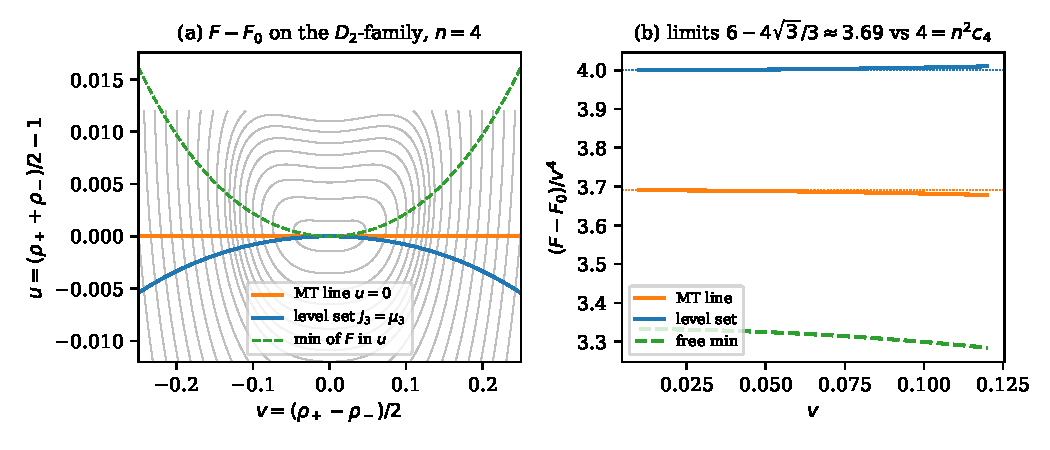
\includegraphics[width=\textwidth]{figures/mt_line.pdf}
\caption{$n=4$ at $b_4=2-\sqrt3$, on the family $\rho_\pm=1+u\pm v$. (a) Contours of $F-F_0$ with MT's
line $u=0$, the momentum level set $J_3=\mu_3$ (which bends to $u\approx u_2v^2$), and, dashed, the curve of
minima of $F$ in $u$ at fixed $v$ (no momentum constraint). (b) $(F-F_0)/v^4$ along the three curves. The
line tends to $D=6-\tfrac43\sqrt3\approx3.691$, the level set to $n^2c_4=4$, and the free minimum to
$D-B^2/(4A)=10/3$. \status{Numerical} \code{code/make_figures.py}.}
\label{fig:mtline}
\end{figure}

\paragraph{Discussion.} Both quartics are positive for every $n$ in Table~\ref{tab:mtline}, so MT's
conclusion for even $n$ is correct; but the quantity they show to be positive is not the reduced quartic,
and the bending term can have either sign (positive at $n=4$, negative for $n\ge6$ in the table). For
example, at $n=4$ the straight line underestimates the reduced quartic by $8\%$, and at $n=20$ it
overestimates it by $55\%$. A positive line value would not in general imply a positive reduced quartic.

Two further observations, stated with less confidence. (i) MT print the $t^4$ coefficient as
$\frac{n}{768\pi r_0^4\sigma^4}T$ with an explicit bracket $T$. Expanding the function $f$ they display, we
find (\status{Certified}, same script) $T_{\rm direct}=n^2(n^2-16)(1+\lambda)^4+48(n-1)(9\lambda^4-14\lambda^3+26\lambda^2+2\lambda+1)$
at $r_0=1$, and $T_{\rm printed}-T_{\rm direct}=72(n-1)\lambda^2(\lambda^2-6\lambda+1)$. MT's printed
closed forms for $T_1+T_2$ and $T_1T_2$ agree with their printed $T$. At $n=4$ the printed $T$ gives $3.6236$
instead of $3.6906$. We have not determined whether this is a typographical or an algebraic slip; it does
not affect the sign. (ii) MT's odd-$n$ criterion $\beta_{\rm MT}\delta_{\rm MT}>\gamma_{\rm MT}^2$~\cite[(3.9)]{MT} also minimises over
$b\in V_1'\subset N$, i.e.\ on the linear slice. The minimum of $F$ on the linear slice
$x_0+\ker dJ(x_0)$ (with the kernel coordinate fixed) differs from $c_4$: in our normalisation it is
$0.2307$, $2.2779$, $2.5781$, $10.9142$ against $c_4=0.25$, $1.6964$, $1.5833$, $6.4904$ for $n=4,8,9,13$
(\status{Numerical} \code{code/c4_slice.py}). We have not recomputed MT's $\beta_{\rm MT},\gamma_{\rm MT},\delta_{\rm MT}$ themselves,
so we do not claim that their odd numbers are those linear-slice values.

%======================================================================
\section{Nonlinear stability at a degenerate minimum}\label{sec:nonlinear}
%======================================================================

That a strict local minimum of the reduced Hamiltonian implies Lyapunov stability modulo $G_\mu$ is the
energy--momentum method; it requires no definiteness of the Hessian. See Patrick~\cite{Patrick92} for the
dynamic interpretation on the reduced space, Ortega and Ratiu~\cite{OR99,OR04} and Patrick, Roberts and
Wulff~\cite{PRW} for general statements (including noncompact groups, with $G_\mu$ compact), and
Montaldi~\cite{Montaldi97}. We claim no novelty here. Because the plane's momentum map is not equivariant
and we want the result for perturbations of arbitrary momentum, we record a short self-contained version
adapted to the present situation; its abstract core is checked in Lean.

\paragraph{Hypotheses.} $(P,\Omega)$ is symplectic, $H$ smooth, a Lie group $G$ acts symplectically
preserving $H$, and $J_1,J_2,J_3$ are Hamiltonians for generators $\xi_1,\xi_2,\xi_3$, with $\xi_3$
generating a circle action $K$ and $\operatorname{span}(\xi_1,\xi_2)$ invariant under $\operatorname{Ad}_K$.
$x_0$ is a relative equilibrium: $dF(x_0)=0$ for $F=H-\omega_0J_3$. Assume:
\begin{itemize}
\item[(A1)] $J_1(x_0)=J_2(x_0)=0$, $K$ rotates $(J_1,J_2)$, and $\{J_1,J_2\}(x_0)\ne0$;
\item[(A2)] $K$ acts freely near $x_0$;
\item[(A3)] there is a smooth curve $j\mapsto x_j$ of relative equilibria through $x_0$ with $J_1=J_2=0$ and
$J_3(x_j)=\mu_3+j$;
\item[(A4)] on $M_\mu=J^{-1}(\mu)/K$, $h_\mu$ has positive semidefinite Hessian at $[x_0]$, definite on a
complement $E$ of its kernel $Z_0$, and $g(a)=\min_yh_\mu(a,y)-h_\mu(0)$ has zero cubic term and positive
definite quartic term.
\end{itemize}

\begin{theorem}\label{thm:abstract}
Under (A1)--(A4), $K\cdot x_0$ is Lyapunov stable in $P$, for perturbations of arbitrary momentum.
\end{theorem}

\begin{proof}
\emph{Lemma A (cross-section).} By (A1), $S=\{J_1=J_2=0\}$ is near $x_0$ a $K$-invariant symplectic
submanifold of codimension~$2$ ($dJ_1,dJ_2$ are independent and $\Omega(X_{J_1},X_{J_2})\ne0$), invariant
under the flow, on which the flow is that of $H|_S$. The implicit function theorem applied to
$(x,s)\mapsto(J_1,J_2)(\exp(s_1\xi_1+s_2\xi_2)x)$, whose $s$-derivative at $(x_0,0)$ is invertible by (A1),
gives a continuous, $K$-equivariant $\Lambda:U\to G$ on a $K$-invariant neighbourhood $U$ of $K\cdot x_0$
with $\Lambda(x)x\in S$ and $\Lambda=e$ on $K\cdot x_0$ (uniqueness of the small solution makes the local
definitions on $K$-translates agree).

\emph{Lemma B1.} In coordinates $(a,y)\in Z_0\times E$ on $M_\mu$, there are $c_1,\varrho>0$ with
$h_\mu(a,y)-h_\mu(0)\ge c_1(|a|^4+|y|^2)$ for $|(a,y)|<\varrho$. Indeed
$h_\mu(a,y)-g(a)-h_\mu(0)\ge c|y-y^*(a)|^2$ by Taylor's theorem in $y$, $g(a)\ge c'|a|^4$ by (A4), and
$|y|^2\le2|y-y^*(a)|^2+2L^2|a|^4$.

\emph{Lemma B2.} By (A2) $S/K$ is a manifold near $[x_0]$. The function $J_3$ is $K$-invariant and descends
to it with nonzero differential: on the symplectic manifold $S$ its Hamiltonian vector field is the
generator of $K$, which is tangent to $S$ and nonzero by (A2), so $dJ_3|_S\ne0$, and $dJ_3|_S$ vanishes on the
orbit direction. Hence $J_3$ is a submersion on $S/K$ near $[x_0]$, and its level sets near $[x_0]$ are the
reduced spaces. Choose coordinates $(j,w)$, $j=J_3-\mu_3$, with $\{w=0\}$ the
curve of (A3) (transverse to the levels since $J_3(x_j)=\mu_3+j$) and $\{j=0\}=M_\mu$ carrying the coordinates of B1. Let $\Phi(j,w)=H(j,w)-H(j,0)$. Since
$x_j$ is critical for $H$ on its level, $\Phi(j,0)=0$ and $\partial_w\Phi(j,0)=0$, hence
$|\partial_j\Phi(0,w)|\le L'|w|^2$ and
$\Phi(j,w)\ge\Phi(0,w)-L'|j|(|a|^2+|y|^2)-C_2j^2$. With B1 and $L'|j||a|^2\le\frac{c_1}2|a|^4+\frac{L'^2}{2c_1}j^2$,
$\Phi\ge\frac{c_1}2(|a|^4+|y|^2)-Cj^2$ near $0$.

\emph{Lemma B3.} $V=H-\omega_0J_3+c_{\rm p}(J_3-\mu_3)^2$ is conserved and $K$-invariant on $S$. Writing
$V-V_0=\Phi+\psi(j)+c_{\rm p}j^2$ with $\psi(j)=H(x_j)-H(x_0)-\omega_0j=O(j^2)$ (because $\frac d{dj}H(x_j)=\omega(j)$),
$V-V_0\ge\frac{c_1}2(|a|^4+|y|^2)+(c_{\rm p}-C-C_3)j^2$, a strict minimum on $S/K$ at $[x_0]$ for $c_{\rm p}$ large.

\emph{Lemma B4.} A conserved continuous function with a strict minimum modulo the compact orbit
$K\cdot x_0$ gives Lyapunov stability of $K\cdot x_0$ for the flow on $S$; solutions stay in a compact
collision-free set and so exist for all time.

\emph{Conclusion.} For $x(0)$ near $K\cdot x_0$ let $g_0=\Lambda(x(0))$. Since $G$ commutes with the flow,
$\tilde x(t)=g_0x(t)$ is the solution through $g_0x(0)\in S$, which stays near $K\cdot x_0$ by B4, and
$\operatorname{dist}(x(t),K\cdot x_0)\le\operatorname{dist}(\tilde x(t),K\cdot x_0)+\sup d(g_0^{-1}z,z)$, the
supremum over $z$ in a compact neighbourhood of $K\cdot x_0$, which tends to $0$ as $g_0\to e$.
\end{proof}

\noindent\status{Proved}. \status{Lean} for the abstract core, in a metric-space setting with the chart,
slice and slaving map as hypotheses: \lean{Conj13.LyapunovAnalytic}: \lean{lemma_B1} (from the existence
of $y^*$ and the slaving inequality), \lean{lemma_B2}, \lean{lemma_B3}; \lean{Conj13.LyapunovAbstract}:
\lean{lyapunov_on_section} (B4) and \lean{stable_modulo_orbit} (the conclusion, for a topological group
acting continuously, given a map $\Lambda$ as in Lemma~A and $G$-equivariant trajectories). These are stated
for trajectories defined on a time interval $I(x)\ni0$, which is the situation of the vortex flow, whose
solutions are a priori only local; that they exist for all time is the last step of B4, by hand (they stay in
a compact collision-free set). Not in Lean: Lemma~A itself, the manifold structure of $S/K$ and the chart,
the existence of $y^*$, global existence, and the vortex flow.

\begin{remark}
The penalty term in B3 is needed in every geometry except the plane. With $\lambda$ fixed, the ring at
momentum $\mu_3+j$ has radius $r$ with $J_3=nr^2/(1+\lambda r^2)$ increasing in $r$, so its parameter
$b=\lambda r^2$ moves away from $b_n$: on the sphere ($n=4,5,6$, $\lambda>0$) $b>b_n$ for $j>0$, and on the
hyperbolic plane ($n\ge8$, $\lambda<0$) $b>b_n$ for $j<0$. Since $C_1(b)=2(n-1)(1+b^2)/(1+b)^2$ is strictly
decreasing on $(-1,1)$, the kernel eigenvalue $\alpha_{\floor{n/2}}=C_1(b)-\floor{n^2/4}$ is then negative and the
ring is a saddle of the reduced Hamiltonian at that momentum (\status{Proved}, from
Proposition~\ref{prop:blocks}); the bifurcated minima have depth $O(j^2)$. So the reduced Hamiltonians at
nearby momenta do not have uniform strict minima, and B2 only bounds how far below zero $\Phi$ can go. In the
plane ($n=7$) $b=0$ for every $r$, the ring stays at the threshold, and the penalty is harmless but not needed.
\end{remark}

\begin{remark}[The free minimum gives no certificate from $D$]
On the family~\eqref{eq:Fuv}, minimising $F$ over $u$ with no momentum constraint gives the quartic
$D-B^2/(4A)$ (Figure~\ref{fig:mtline}(a), dashed). It is a lower bound for both MT's line value $D$ and the
level-set value $D+Bu_2+Au_2^2$, since $A>0$. At $n=4$ it is $10/3\approx3.333$ (against $D\approx3.691$ and $4$),
at $n=8$ it is $751/7\approx107.29$ (against $145.79$ and $108.57$) (\status{Certified} \code{code/mt_line_vs_levelset.py}).
Positivity of $D$ therefore bounds nothing from below; positivity of the free minimum would, within this
family.
\end{remark}

\paragraph{Proof of Theorem~\ref{thm:main}.} We check (A1)--(A4) for the ring at $b_n$, $n\ge4$, in all three
geometries. (A1): $J_+(x_0)=0$ by $\Z_n$-symmetry, a rotation by $\psi$ multiplies $J_+$ by $e^{i\psi}$,
$\{J_1,J_2\}(x_0)=n(1-b_n)/(2(1+b_n))\ne0$ since $|b_n|<1$ (Proposition~\ref{prop:bn}), and
$\operatorname{span}(\xi_1,\xi_2)$ is $\operatorname{Ad}_K$-invariant in $\mathfrak{so}(3)$, $\mathfrak{se}(2)$
and $\mathfrak{sl}(2,\R)$. (A2): a nontrivial rotation moves a labelled ring. (A3): the concentric rings
of radius $r$ are relative equilibria with $J_+=0$ and $J_3=nr^2/(1+\lambda r^2)$ strictly increasing in
$r$. (A4): Proposition~\ref{prop:spectral}, Lemma~\ref{lem:sym}, and $c_4>0$ by Theorems~\ref{thm:even}
and~\ref{thm:odd}; the quartic term of $g$ is $c_4|a|^4$ in the chart of Definition~\ref{def:c4}, and by
Lemma~\ref{lem:chart} its positivity is chart-independent. Theorem~\ref{thm:abstract} gives
Theorem~\ref{thm:main}. Since $K$ is compact, $K$-invariant neighbourhoods of $K\cdot x_0$ are cofinal,
so this is stability in MT's sense~\cite[p.~10]{MT}. \qed

\noindent\status{Proved} (the instantiation). The facts used are Lean-checked as cited above, except the
reduced-space structure, the Poisson structure of $\Omega$ and the vortex flow, which are by hand.

%======================================================================
\section{A direct integration}\label{sec:numerics}
%======================================================================

As a check on the theory (not part of the proof), we integrated the $n=8$ ring in the hyperbolic plane
(Poincar\'e disk of curvature $-1$, DOP853, relative tolerance $10^{-12}$, $T=2000$). With $\zeta=\sqrt{-\lambda}\,z$,
MT's chart for $\lambda<0$ becomes the curvature $-1$ Poincar\'e disk, $\sigma=1-|\zeta|^2$, and $\Omega$ becomes a
constant multiple of its area form; a ring of radius $r_0$ has $\xi:=|\zeta|^2=-\lambda r_0^2=-b$. So the
threshold is $\xi^*=-b_8=8-3\sqrt7$, and $\mathrm{rel}>0$ in $\xi=\xi^*(1+\mathrm{rel})$ means $b<b_8$, the
linearly stable side. We start from the ring at $\xi=\xi^*(1+\mathrm{rel})$ plus the critical mode with relative
amplitude $\delta=10^{-3}$ (Figure~\ref{fig:n8}). The diagnostic $\mathcal D(t)=\max_{i<j}|d_{ij}(t)-d_{ij}^{\rm ring}|$ uses hyperbolic
distances and is invariant under the whole group. On the linearly unstable side the deviation grows to an
amplitude that scales like $\sqrt{|\mathrm{rel}|}$ (the stable bifurcated $n/2$-gon pair of a supercritical
pitchfork); at the threshold and on the stable side $\max_t\mathcal D(t)/\mathcal D(0)=1.000$ to three decimals, with no
secular growth. \status{Numerical}: the traces in Figure~\ref{fig:n8} are recorded outputs of the original
integration (not rerun); \code{code/n8_integration.py} reruns the same experiment and prints the maxima.

\begin{figure}[t]
\centering
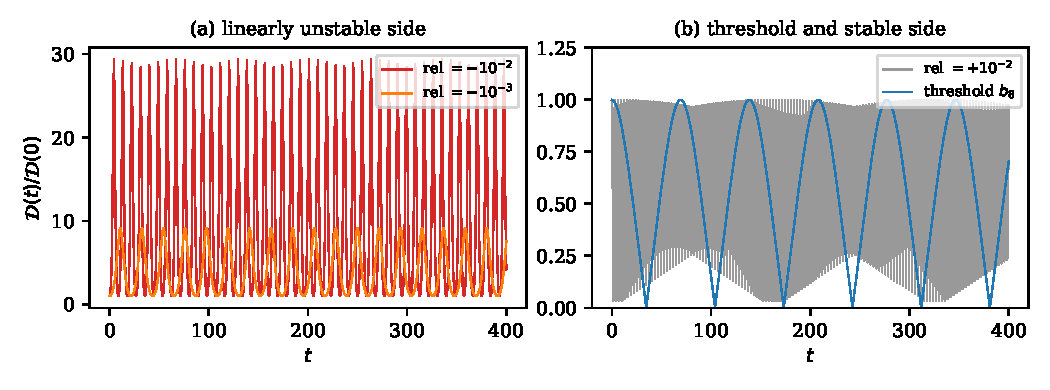
\includegraphics[width=\textwidth]{figures/n8_traces.pdf}
\caption{$n=8$, hyperbolic plane: $\mathcal D(t)/\mathcal D(0)$ for a critical-mode perturbation $\delta=10^{-3}$ of the ring
at relative offset rel from the threshold. (a) Unstable side: the orbit wanders near the bifurcated pair.
(b) Threshold (blue) and stable side (grey): the deviation never exceeds its initial value.
\status{Numerical}.}
\label{fig:n8}
\end{figure}

%======================================================================
\section{Relation to prior work}\label{sec:prior}
%======================================================================

\paragraph{Montaldi--Tokieda~\cite{MT}.} We quote arXiv:1210.5662v1 (the only arXiv version); we did not
consult the published chapter (Springer, 2013, pp.~335--370), so page and equation numbers, the bracket
$T$ and Proposition~9 are as in the arXiv text. MT introduce the family, prove linear stability below $b_n$ and
instability above, identify the pitchfork, and pose Conjecture~13. At the threshold they treat even $n$ by
the straight-line quartic of Section~\ref{sec:mt} (with Maple closed forms for $T_1+T_2$ and $T_1T_2$),
$n=5,9,11$ by 2--4 significant-digit evaluations of their coefficients $\beta_{\rm MT},\gamma_{\rm MT},\delta_{\rm MT}$, $n=7$ by Maple, and $n=3$ by a
remark. Our symmetry argument for the absence of a cubic term on the kernel is theirs~\cite[Prop.~12]{MT}.

\paragraph{The heptagon.} For $n=7$ (the plane) nonlinear stability is due to Kurakin and Yudovich~\cite{KY}
and Schmidt~\cite{Schmidt}; MT recover it~\cite[Cor.~7]{MT}. Our $n=7$ case is a special case of the uniform
argument.

\paragraph{Critical cases elsewhere.} Kurakin~\cite{Kurakin10} carries out a critical-case Lyapunov analysis
for the regular $n$-gon inside a circular domain. For the sphere, Borisov and Kilin~\cite{BK} note that the
critical latitude needs a separate nonlinear analysis, and Kurakin~\cite{Kurakin03,Kurakin04} gives
conditions for nonlinear stability of regular vortex systems on the sphere. Constantineau,
Garc\'\i a-Azpeitia, Garc\'\i a-Naranjo and Lessard~\cite{CGGL} give computer-assisted proofs of the
stability of branches of relative equilibria on the sphere bifurcating from the rings, away from the
degenerate point, not at the threshold itself.

\paragraph{Energy--momentum method.} The step from a strict minimum of the reduced Hamiltonian to Lyapunov
stability modulo $G_\mu$ is standard~\cite{Patrick92,OR99,OR04,PRW,Montaldi97}; Section~\ref{sec:nonlinear}
only adapts it.

\paragraph{What is new here.} To our knowledge (we have not found these in the literature):
(i) a proof of Conjecture~13 uniform in $n\ge4$, in particular for all odd $n\ge13$; (ii) the exact closed forms
of the level-set quartic $c_4$ for all $n$; (iii) the observation that MT's even-$n$ quartic is taken off the
momentum level set and differs from the reduced quartic, with the exact correction
(Proposition~\ref{prop:mtline}); (iv) machine-checked proofs of the algebraic and series steps.

%======================================================================
\section{Status and limitations}\label{sec:status}
%======================================================================

\paragraph{Review status.} \textbf{No human specialist has refereed this argument.} It has been
checked by computer, including independent re-derivations (Lean, exact symbolic and modular computation,
high-precision numerics), and by AI-assisted adversarial review. Its claims should be treated
accordingly.

\paragraph{What Lean checks.} Library \lean{Conj13} in \code{lean/Conj13/} of the accompanying repository
(Lean 4, Mathlib v4.34.1), with no \lean{sorry} and only the standard axioms \lean{propext},
\lean{Classical.choice}, \lean{Quot.sound} (\code{outputs/lean_axioms.out}):
\begin{itemize}
\item the threshold $b_n$: closed form, uniqueness, sign pattern (Proposition~\ref{prop:bn});
\item the spectral picture: from the Hamiltonian, that the ring is critical exactly for $\omega_0$ and
that the Hessian is block-diagonal over Fourier modes with blocks $\operatorname{diag}(\alpha_m,\beta_m)$, for every
$b>-1$; the Fej\'er identity for all $n$, the factorisation and sign of $\alpha_m$, the $V_1'$ eigenvalues
(Propositions~\ref{prop:blocks},~\ref{prop:spectral});
\item the partial derivatives and the value of $\{J_1,J_2\}$ (Section~\ref{sec:reduced});
\item the invariant-monomial arithmetic of Lemma~\ref{lem:sym};
\item for even $n$, starting from the Hamiltonian of $n$ labelled points: the product formula, that the
staggered curve lies in $J^{-1}(\mu)$ and in the gauge, its jet, the normalisation, and the limit
$(H-H_0)/\varepsilon^4\to c_4$ at $b_n$ for every $n$;
\item for odd $n$, again from the Hamiltonian: the full fourth-order jet along the ansatz (including the
pair sums via first- and second-order Fej\'er identities and the absence of the $A^3$ term), the $J_1$
constraint, the normalisation, and the constrained minimisation and its reduction modulo the threshold;
\item the closed forms of $c_4$ at the true $b_n$, their positivity for every $n\ge4$, and Table~\ref{tab:c4};
\item the straight-line jet of $F$ and the jets on every curve $u=\kappa v^2$ (both from the
Hamiltonian, which identifies $A$, $B$, $D$ and $u_2$), the bending identity, and the $n=4$ comparison
(Proposition~\ref{prop:mtline}, Corollary~\ref{cor:n4});
\item the abstract Lyapunov argument (Lemmas B1--B4 and the conclusion of Theorem~\ref{thm:abstract}),
with the slice, the chart and the slaving map as hypotheses.
\end{itemize}

\paragraph{What is by hand.} The reduced space and the restriction of the Hessian to $\ker dJ$
(Proposition~\ref{prop:spectral}; the momentum differentials and $V_1'$); the identification of the
polarised second derivatives with the Hessian matrix; the Poisson structure of $\Omega$ (taken as a
definition in the bracket computation); the chart-independence and symmetry lemmas; symmetric criticality
for even $n$; the completeness of the odd ansatz (which modes are slaved at order $A^2$, the reflection
symmetry, the irrelevance of $O(A^3)$ corrections) and the identification of the constrained minimum with
the quartic of $g$; Lemma~A, the manifold chart on $S/K$ and the slaving map; and the instantiation of
Theorem~\ref{thm:abstract} for the vortex flow (existence of solutions, conservation laws). These
steps are supported independently by the exact $\mathrm{GF}(p)$ Cartesian KKT computation (no ansatz, no
symmetry reduction) and by the high-precision numerics, but those are not proofs.

\paragraph{Scope.} The result concerns MT's family~\eqref{eq:H}, i.e.\ the ``sinh'' interaction on the
hyperbolic plane. The same method extends to other hyperbolic interactions (for instance the
image or ``tanh'' kernel) and to interpolating families; we do not treat them here. We do not address the
bifurcated branches, KAM-type questions, or $n=3$.

\section*{Acknowledgement and disclosure of AI assistance}
This work was developed with substantial assistance from an AI system (Claude, Anthropic), covering the
derivations, the Lean formalisation, the computer-algebra and numerical code, and the drafting of this
manuscript; the author directed the work and takes responsibility for the content. No human expert has yet
checked the mathematics, and corrections are welcome. We thank James Montaldi and Tadashi Tokieda, whose
paper posed the problem and supplied the framework used here.

\appendix
\section{Coefficients for odd \texorpdfstring{$n$}{n}}\label{app:odd}

Along the ansatz of Theorem~\ref{thm:odd}, $H-H_0=f_2A^2+E(p,s)A^4+O(A^5)$ with
$E=E_{00}+E_{10}p+E_{01}s+E_{20}p^2+E_{02}s^2$ (no $ps$ term) and
\begin{align*}
E_{20}&=\tfrac1{16}n(n-1)(1-\lambda)^2(1+\lambda)^2, &
E_{02}&=\tfrac14n(n-1),\\
E_{10}&=\tfrac1{64}n(n-1)(1-\lambda)(1+\lambda)^3\big[(n-5)(1+\lambda^2)+2(n-1)\lambda\big], &
E_{01}&=\tfrac1{64}n(n-1)^2(1+\lambda)^4,
\end{align*}
\begin{multline*}
E_{00}=\tfrac{n(n-1)(1+\lambda)^4}{8192}\Big[(n^3+n^2-69n+291)(1+\lambda^4)
+4(n^3+n^2-21n-13)(\lambda+\lambda^3)\\+(6n^3+6n^2-30n+82)\lambda^2\Big].
\end{multline*}
The constraint is $\tfrac{1-\lambda}2p-\tfrac{1}{1+\lambda}s-\tfrac{(1+\lambda)^3}{16}=0$. Eliminating $s$, the
coefficient of $p^2$ is $a_2=\tfrac18n(n-1)(1-\lambda)^2(1+\lambda)^2$.
\status{Lean}: \lean{Conj13.Odd4Hamiltonian}: \lean{Ham_oddAnsatz_jet} derives this jet, with exactly these coefficients
(definitions \lean{E00}, \dots, \lean{E02}, \lean{Efun} in \lean{Conj13.Algebra}), from the Hamiltonian;
\lean{J1con}, \lean{E_vertex}, \lean{odd_min_value}, \lean{c4odd_reduction} do the elimination.

\section{Expansions behind \texorpdfstring{$h_4$}{h4} and the \texorpdfstring{$E_{ij}$}{Eij}}\label{app:expansions}

These are the steps a reader needs to reproduce the coefficients by hand; Lean checks each of them
(\lean{Conj13.EvenCurve}: \lean{Phi_jet}; \lean{Conj13.Odd4Pair}: \lean{jet_logPw}, \lean{jet_pair};
\lean{Conj13.Odd4Fejer}).

\paragraph{Even $n=2M$.} On the curve $\mathcal G(u_\pm)=\mathcal G(1)\pm\tau$ one has, with $x=(1+b)\tau$,
$u_\pm=(1\pm x)/(1\mp bx)$ and $1+bu_\pm=(1+b)/(1\mp bx)$. Hence $\log u_++\log u_-=\log(1-x^2)-\log(1-b^2x^2)$,
$\log u_+-\log u_-=2(\operatorname{artanh}x+\operatorname{artanh}bx)$, and the product formula of
Theorem~\ref{thm:even} becomes
\[
H-H_0=-\tfrac{M(2M-1)}2\big[\log(1-x^2)+\log(1-b^2x^2)\big]-2M\log\cosh Y,\qquad
Y=\tfrac M2\big(\operatorname{artanh}x+\operatorname{artanh}bx\big),
\]
using $\log\big((u_+^{M/2}+u_-^{M/2})/2\big)=\tfrac M4(\log u_++\log u_-)+\log\cosh\big(\tfrac M4(\log u_+-\log u_-)\big)$.
Insert $\log(1-x^2)=-x^2-\tfrac12x^4$, $Y=c_1x+c_3x^3$ with $c_1=\tfrac M2(1+b)$, $c_3=\tfrac M6(1+b^3)$, and
$\log\cosh Y=\tfrac12c_1^2x^2+(c_1c_3-\tfrac1{12}c_1^4)x^4$, all up to $O(x^6)$. The $x^2$ and $x^4$
coefficients, multiplied by $(1+b)^2$ and $(1+b)^4$, are $h_2$ and $h_4$.

\paragraph{Odd $n$.} In canonical coordinates $|z_i-z_j|^2/(\sigma_i\sigma_j)=D_{ij}$ with
$D_{ij}=w_i+w_j-2\lambda w_iw_j-2Q_iQ_j\cos\Theta_{ij}$, $Q_k=\sqrt{P(w_k)}$, $P(w)=w(1-\lambda w)$,
$\Theta_{ij}=\vartheta_j-\vartheta_i$. Along the ansatz write $w_k=w_0+e_kA+f_kA^2$ with
$e_k=\cos(l\phi_k)$, $f_k=p\cos\phi_k$, and $\Theta_{ij}=\theta+A^2d$ with $\theta=\phi_j-\phi_i$,
$d=s(\sin\phi_j-\sin\phi_i)$. Factor $D=2Q_iQ_j(K+Y)$ with $K=1-\cos(\theta+A^2d)$ and
$Y=(w_i+w_j-2\lambda w_iw_j)/(2Q_iQ_j)-1=O(A^2)$. Then, writing $K_0=1-\cos\theta$,
\[
\log D-\tfrac12\log P_i-\tfrac12\log P_j=\log2+\log K_0+\frac{K_2+Y_2}{K_0}A^2+\frac{Y_3}{K_0}A^3
+\Big(\frac{K_4+Y_4}{K_0}-\frac{(K_2+Y_2)^2}{2K_0^2}\Big)A^4+O(A^5),
\]
with $K_2=d\sin\theta$, $K_4=\tfrac12d^2\cos\theta$, $Y_2=\tfrac18(1+\lambda)^4(e_i-e_j)^2$,
\begin{align*}
Y_3&=\tfrac18(\lambda-1)(1+\lambda)^5(e_i-e_j)^2(e_i+e_j)+\tfrac14(1+\lambda)^4(e_i-e_j)(f_i-f_j),\\
Y_4&=\tfrac{3}{128}(1+\lambda)^6(5\lambda^2-6\lambda+5)(e_i-e_j)^2(e_i^2+e_j^2)
+\tfrac1{64}(1+\lambda)^6(9\lambda^2-14\lambda+9)(e_i-e_j)^2e_ie_j\\
&\quad+\tfrac18(\lambda-1)(1+\lambda)^5(e_i-e_j)^2(f_i+f_j)\\
&\quad+\tfrac14(\lambda-1)(1+\lambda)^5(e_i-e_j)(f_i-f_j)(e_i+e_j)+\tfrac18(1+\lambda)^4(f_i-f_j)^2.
\end{align*}
The one-body term is $\log P(w_0+eA+fA^2)=\log w_0^2+L_1eA+(L_1f+L_2e^2)A^2+(2L_2ef+L_3e^3)A^3
+(L_2f^2+3L_3e^2f+L_4e^4)A^4+O(A^5)$, where $L_1=(1+\lambda)(1-\lambda)$, $L_2=-\tfrac12(1+\lambda)^2(1+\lambda^2)$,
$L_3=\tfrac13(1+\lambda)^3(1-\lambda^3)$, $L_4=-\tfrac14(1+\lambda)^4(1+\lambda^4)$ are the Taylor
coefficients of $\log(1+(1+\lambda)x)+\log(1-\lambda(1+\lambda)x)$. Since each vortex lies in $n-1$ pairs,
\[
H-H_0=-\sum_{i<j}\big[(\log D-\tfrac12\log P_i-\tfrac12\log P_j)-(\cdot)_{A=0}\big]
-\tfrac{n-1}2\sum_k\big[\log P_k-\log w_0^2\big].
\]
Products of cosines and sines of $\phi_i,\phi_j$ are reduced to single frequencies by the product-to-sum
formulas; summing over $i$ at fixed $\theta=\phi_j-\phi_i$ removes every term whose total frequency is not
$\equiv0\pmod n$ (here $2l\equiv-1$ matters), and the remaining sums over $\theta=2\pi m/n$ are
\begin{gather*}
\sum_{m=1}^{n-1}\frac{\cos(q\theta_m)}{1-\cos\theta_m}=\frac{n^2-1}6-q(n-q),\\
\sum_{m=1}^{n-1}\frac{\cos(q\theta_m)}{(1-\cos\theta_m)^2}=\frac{n^4-30n^2q^2+10n^2+60nq^3-60nq-30q^4+60q^2-11}{180}
\end{gather*}
for $0\le q\le n$, together with $\sum_m\cos(q\theta_m)=n[n\mid q]-1$. This yields $f_2$ and the $E_{ij}$ of
Appendix~\ref{app:odd}.

\bibliographystyle{plain}
\bibliography{refs}

\end{document}
